% !TEX root = paper.tex

\section {Results}
\label{sec:results}

\subsection{Ridge yield}

Figure~\ref{fig:PlotCorrMBHMT} shows two-particle correlation functions as functions of the relative pseudorapidity ($\Delta \eta$) and azimuthal angle ($\Delta \varphi$) differences between the trigger and associated particles. The functions are measured with Eq.~\ref{eq:corrfunction} for $1 < \pttrig~\mathrm (\ptassoc) < 2$ GeV/$c$ in pp collisions at $\sqrt{\it{s}} = $\unit{13} {\rm{}TeV}. The left panel is for the 0--0.1\% multiplicity class. The right one is from the minimum bias events (0--100\% multiplicity class). The ridge structure is clearly observed in the high multiplicity class compared to the minimum-bias events while it is not seen in the minimum bias events. The away side is dominant from the correlation of back to back jet.

\begin{figure}[h!]
	\centering
	\subfigure{ 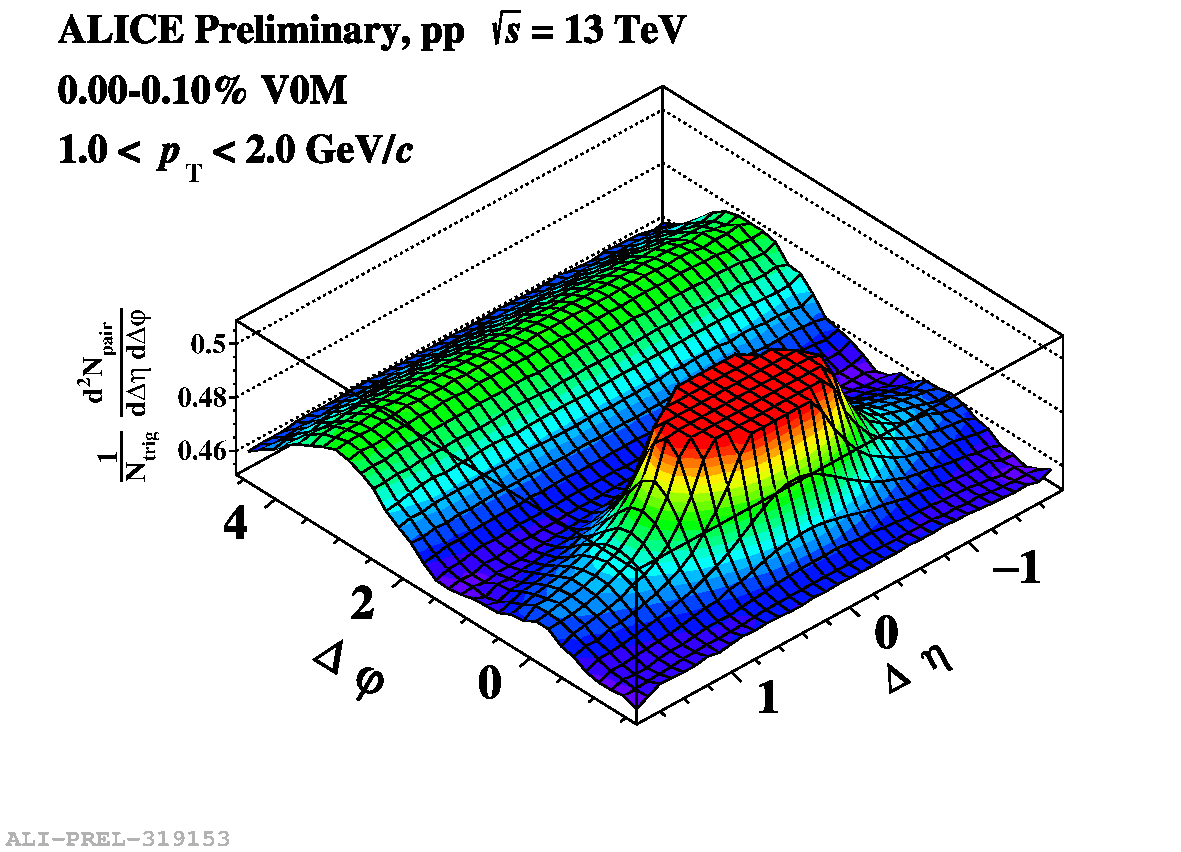
\includegraphics[width=0.47 \textwidth]{./figures/corr1.pdf} }
	\subfigure{ 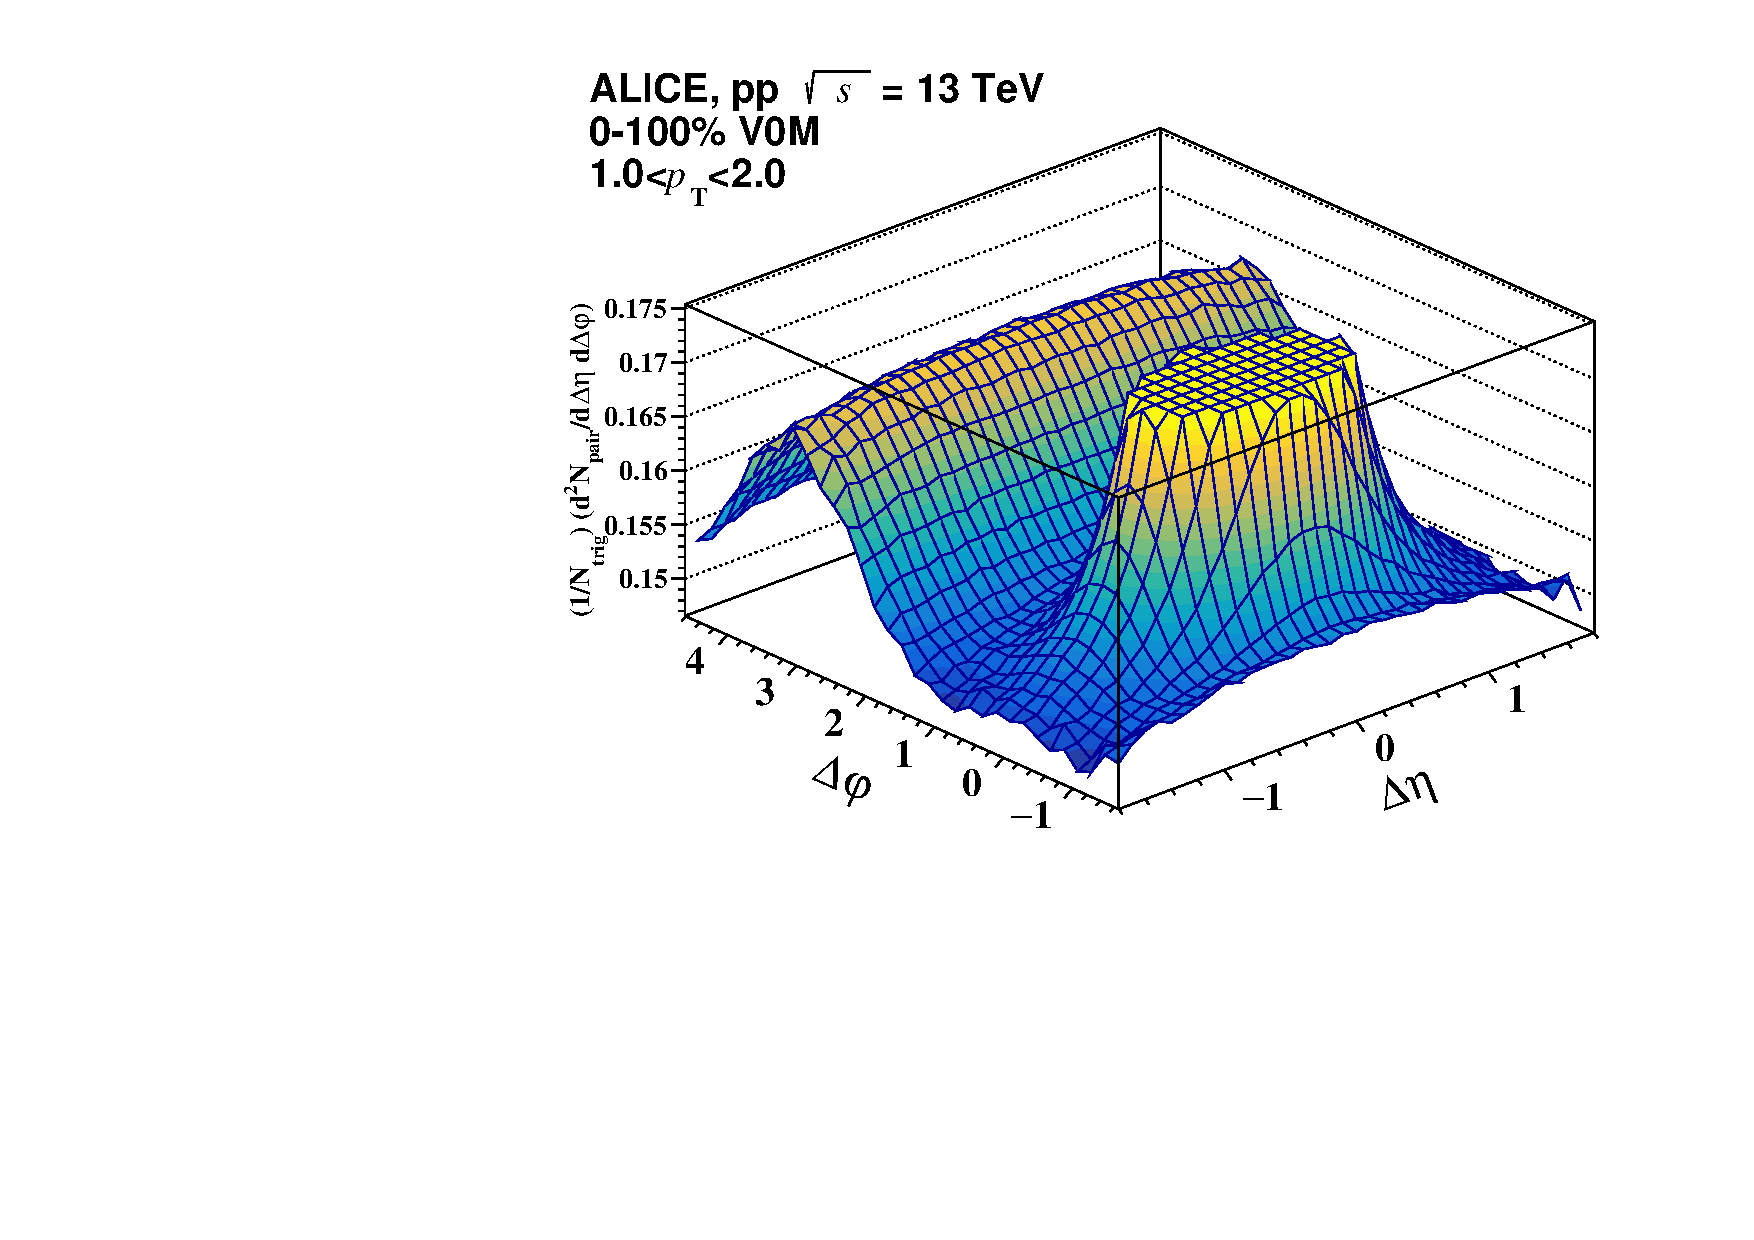
\includegraphics[width=0.47 \textwidth]{./figures/corrmb.pdf} }
	\caption{ Dihadron correlation functions as functions of $\Delta\eta$ and $\Delta\varphi$ in the high multiplicity (0--0.1\%, left) and the minimum-bias events (0--100\%, right). The intervals of $\pttrig$ and $\ptassoc$ are equally $1 < \it{p}_{\rm{T}} < 2$ GeV/$c$. }
	\label{fig:PlotCorrMBHMT}
\end{figure}

 Projected $\Delta\varphi$ distributions of the two-particle correlation functions in $1.6<|\Delta\eta|<1.8$ are shown in Fig.~\ref{fig:PlotDeltaPhi} for various $\it{p}_{\rm{T}}$ intervals in the minimum bias class(0--100\%) and the high multiplicity class (0--0.1\%). The near-side($\Delta\varphi\sim 0$) peak in 0--0.1\% multiplicity class is clearly observed in all the transverse momentum ranges studied while there is no hint of signal in the minimum bias class. The near-side peak is highest in the interval of $1<\it{p}_{\rm{T}}<2$ GeV/$c$ and gradually decreases with increasing $\it{p}_{\rm{T}}$ in the high multiplicity class. The measurements in the high multiplicity class are compared with the results measured by the CMS collaboration~\cite{Khachatryan:2015lva}. The near-side peaks in all transverse momentum ranges are comparable each other within the uncertainties. The larger away yields observed in \cite{Khachatryan:2015lva} can be attributed to the difference in $\eta$ acceptances. The model predictions are presented for the measurements in the high multiplicity class with the same acceptances used in this article both for $\eta$ and event multiplicity. The $\pythiashoving$ gives good estimates of the near-side peak and slightly overestimates the away-side yield for the interval of $1<\it{p}_{\rm{T}}<2$ GeV/$c$. However the $\pythiashoving$ underestimates the near-side peak for the $\it{p}_{\rm{T}}>2$ GeV/$c$ range. $\pythiam$ does not show any peaks in the near-side as expected and slightly underestimates the away-side peak for $1<\it{p}_{\rm{T}}<2$ GeV/$c$ and gives good estimates for the $\it{p}_{\rm{T}}>2$ GeV/$c$ range, which mainly come from the back to back jet correlations.

 %The associated yield per trigger particle is compared with the CMS results. 


\begin{figure}[h!]
	\centering
	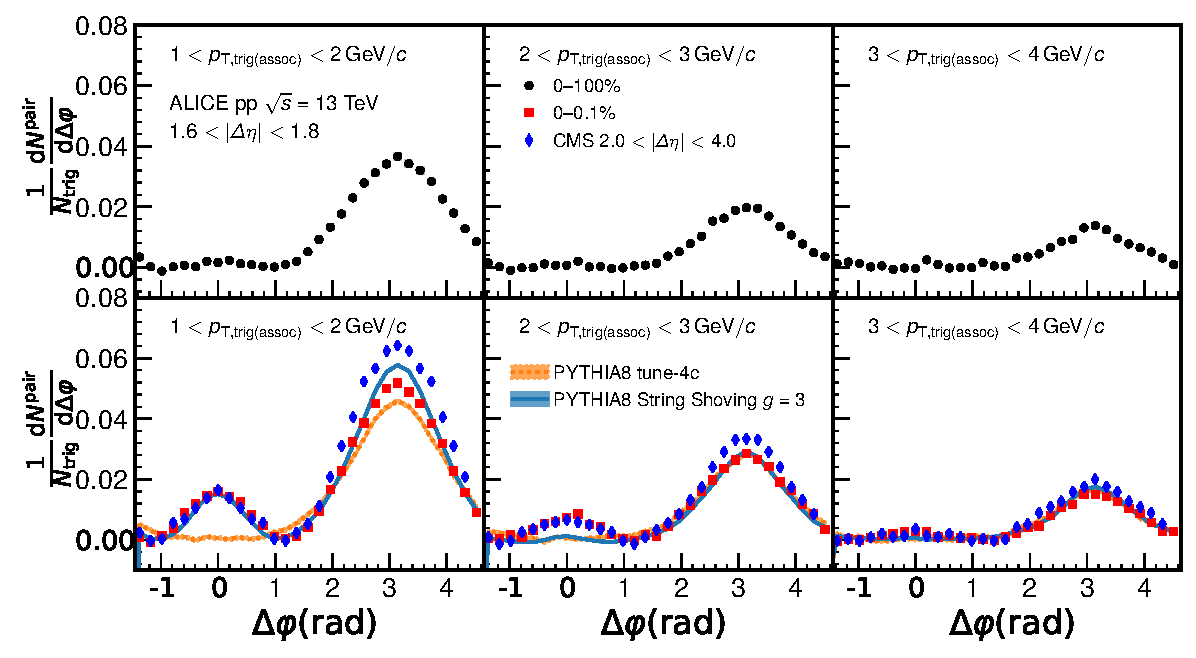
\includegraphics[width=0.99\linewidth]{./figures/Fig2_PlotDeltaPhi.pdf}
	\caption{One-dimensional $\Delta\varphi$ distribution in the large $\Delta\eta$ with various transverse momentum intervals in each multiplicity class. The distributions in upper panels are measured with 0--100\% multiplicity class. The distribution in lower panels are measured with 0-0.1\% multiplicity class. Interval of transverse momentum of trigger particle and associated particle is $1<\pt<2$ (left), $2<\pt<3$ (middle) and $3<\pt<4$ GeV/$c$ (right), respectively. The model predictions are presented as colored lines. Blue line corresponds to the $\pythiashoving$ and orange line corresponds to the $\pythiam$}
	\label{fig:PlotDeltaPhi}
\end{figure}
 
The ridge yields as a function of  the transverse momentum are shown in Fig.~\ref{fig:PlotYSpect} in the high multiplicity class and compared to \cite{Khachatryan:2015lva}. The particle multiplicity in this analysis is estimated with the forward subsystem(V0), whereas that in \cite{Khachatryan:2015lva}  used the mid-rapidity particles in $|\eta|<$2.4 and $\pt>0.4$ GeV/$c$. By interpolating the $\eta$ and $\pt{}$ distributions based on PYTHIA, it is found that the multiplicity in \cite{Khachatryan:2015lva} is about 20\% higher than 0--0.1\% in this analysis, corresponding 0--0.03\%. Taking into account the differences in acceptance of charged tracks and estimated multiplicity, the measurements are comparable with each other. The spectrum is also compared with model calculations. $\pythiam$ gives zero yields since it does not contain the ridge effect. $\pythiashoving$ describes the yield qualitatively however its yield decreases more rapidly than the data as $\pttrigassoc$ increases.

\begin{figure}[h!]
	\centering
	\subfigure{ 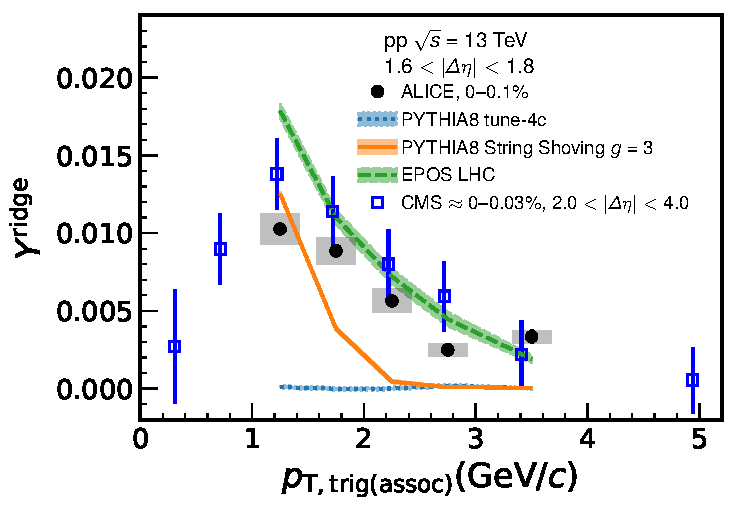
\includegraphics[width=0.89\textwidth]{./figures/Fig3_PlotRidgeYield.pdf} }
	\caption{ The spectra of ridge yield as function of transverse momentum. The filled circles denote the measurement with ALICE and compared with CMS measurement~\cite{Khachatryan:2015lva}, which is represented as open blue box. The two lines show model predictions from $\pythiam$ (orange line) and $\pythiashoving$ (blue line). }
	\label{fig:PlotYSpect}
\end{figure}

\subsection{Event scale dependent ridge yield}
The event scale dependent ridge yields are measured with the minimum $\ptlead=9.0$ (left) or $\ptjet=10.0$~ GeV/$c$ (right) thresholds for $1< \pttrig~\mathrm (\ptassoc) <2$ GeV/$c$, where the measured ridge yield is maximum without event scale selection. In Fig.~\ref{fig:PlotCorrHMTSel}, The ridge structure still persist even with both selections. With the minimum $\ptjet$ selection, the correlations function has double peaks on the $\Delta\eta$ at $\Delta\varphi = \pi$ due to the requirement of the limited jet acceptance.

\begin{figure}[h!]
	\centering
	\subfigure{ 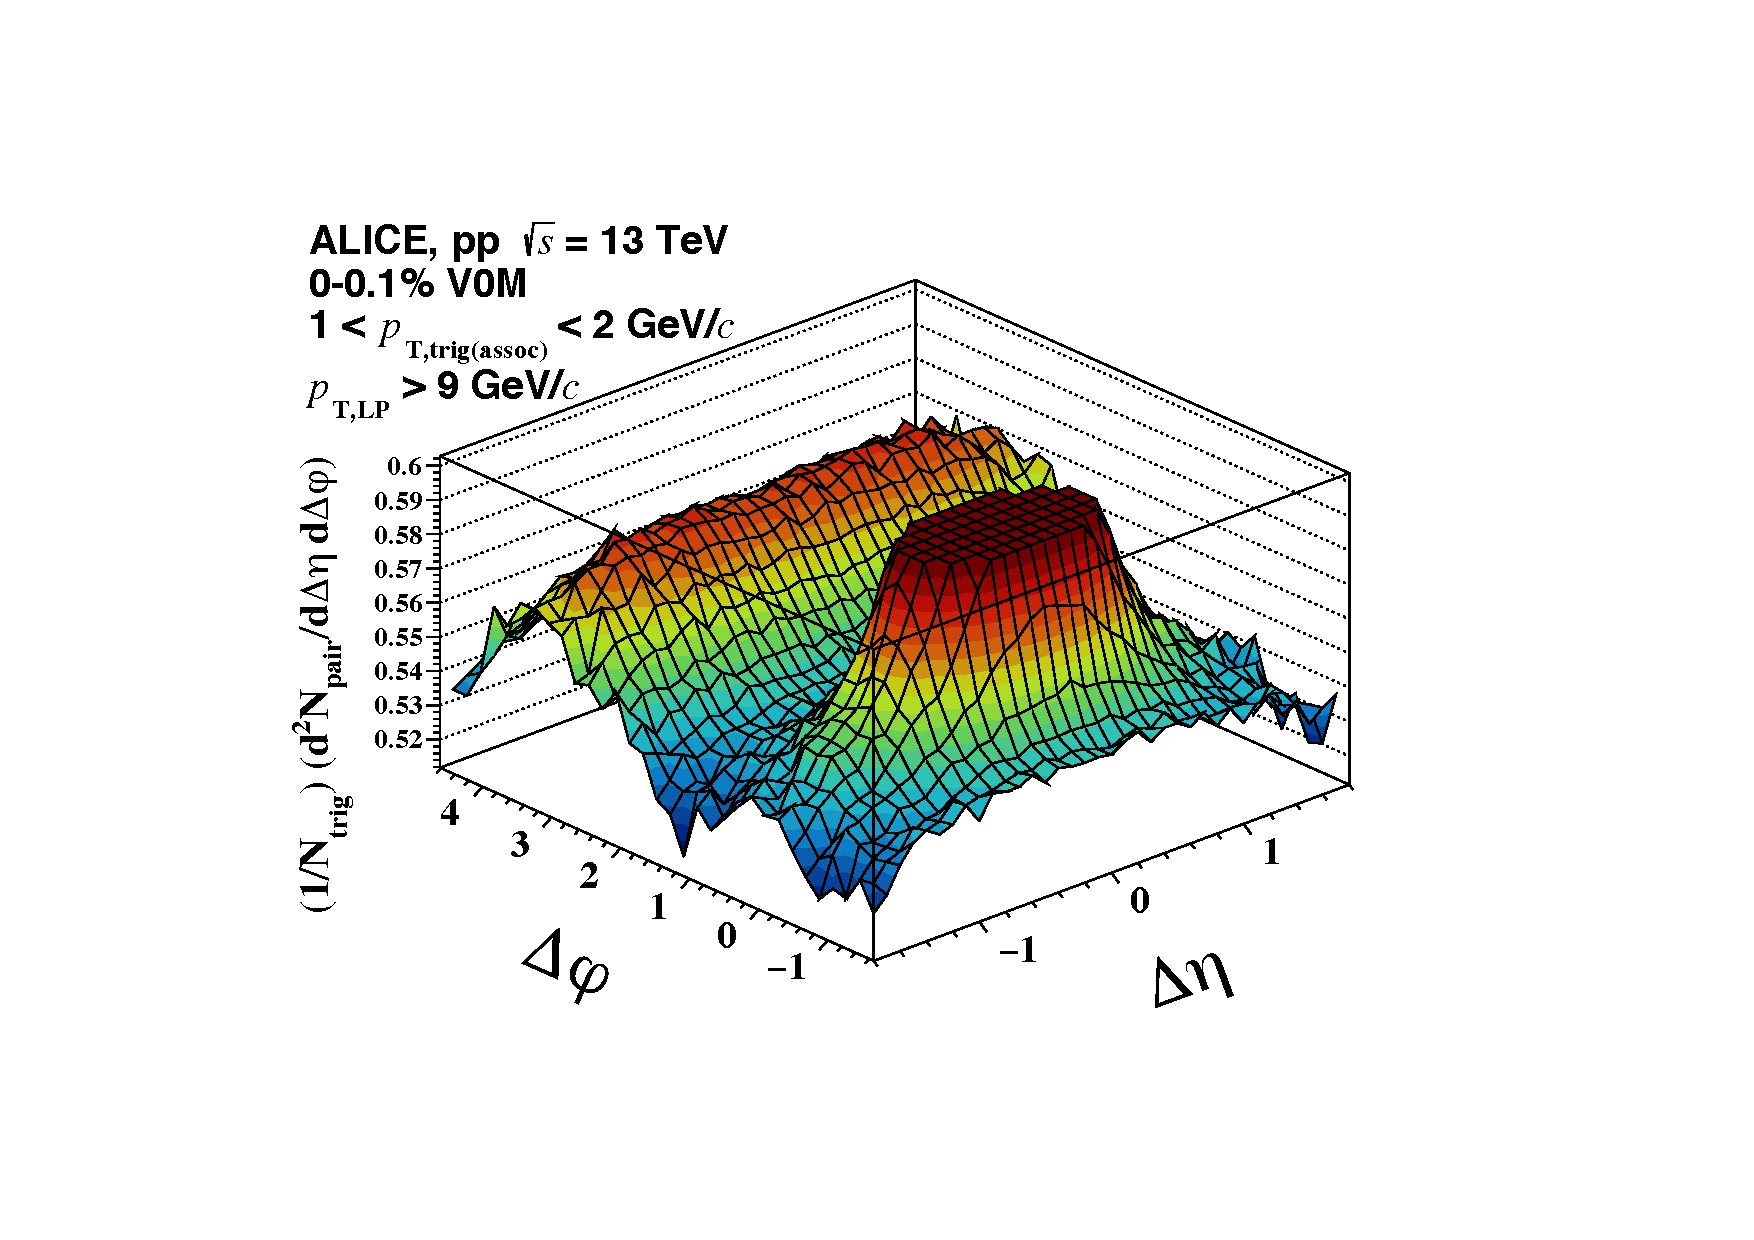
\includegraphics[width=0.47 \textwidth]{./figures/corrlh.pdf} }
	\subfigure{ 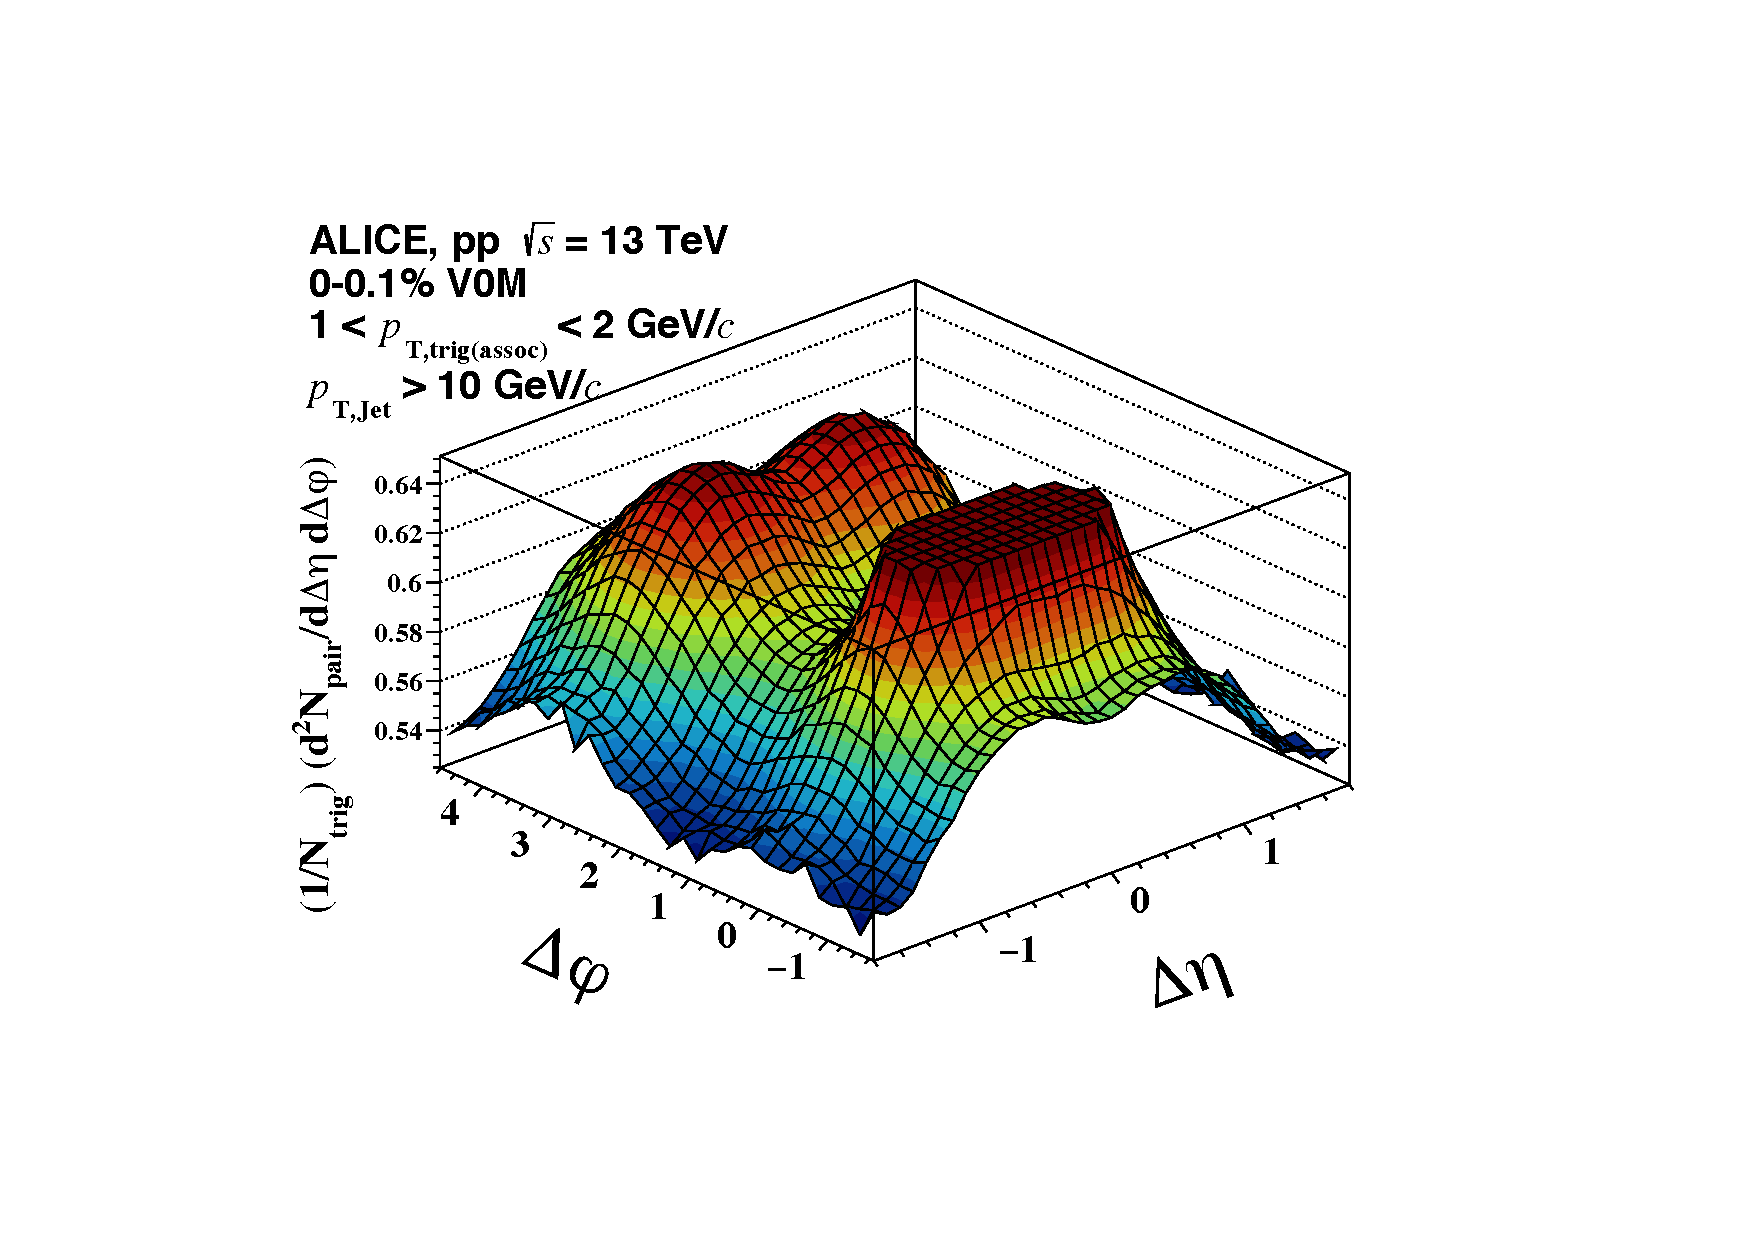
\includegraphics[width=0.47 \textwidth]{./figures/corrjet.pdf} }
	\caption{ Two-dimensional correlations function as function of $\Delta\eta$ and $\Delta\varphi$ in top 0-0.1\% multiplicity class with the minimum $\ptlead$ (left) or $\ptjet$ (right) selection. The interval of $\pttrig$ and $\ptassoc$ is $1<\pt<2$ GeV/$c$. The minimum requirement for $\ptlead$ or $\ptjet$ is 9 and 10 GeV/$c$, respectively. }
	\label{fig:PlotCorrHMTSel}
\end{figure}

Projected $\Delta\varphi$ distributions of the correlation functions in $1.6<|\Delta\eta|<1.8$ with the minimum $\ptlead$(lower) and $\ptjet$(upper) are shown in Fig.~\ref{fig:PlotDeltaPhiESE}. The near-side yield increases as requiring higher $\ptlead$ or $\ptjet$ from the yield in unbiased events, which is shown in the upper left panel. The Model calculations by $\pythiashoving$ and $\pythiam$ are shown with a blue and a orange line, respectively. The $\pythiashoving$ gives qualitative agreement of the near-side peak with the event scale selections. On the other hand, $\pythiam$ does not show the near-side peak with the event scale selections. Both models describe the away-side yield with the $\ptjet$ selection and overestimate away-side yield with the $\ptlead$ selection.

\begin{figure}[h!]
	\centering
	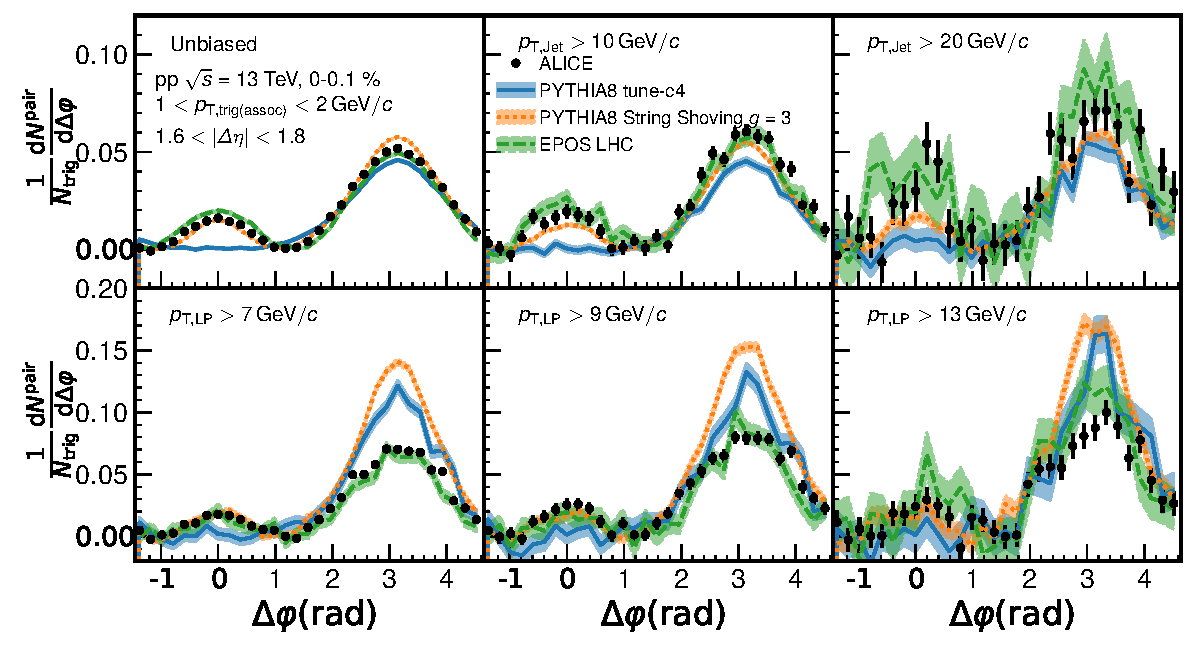
\includegraphics[width=0.99\linewidth]{./figures/Fig5_PlotDeltaPhiESE.pdf}
	\caption{ One-dimensional $\Delta\varphi$ distribution in the large $\Delta\eta$ with the minimum $\ptlead$(lower) or $\ptjet$(upper) selection for $1< \pttrig~\mathrm (\ptassoc) <2$ GeV/$c$ in the 0--0.1\% multiplicity class. The filled circles show measurement with ALICE. Model predictions are compared with measurement with a blue line for $\pythiashoving$  and a orange line for $\pythiam$.}
	\label{fig:PlotDeltaPhiESE}
\end{figure}

The ridge yields as functions of the minimum $\ptlead$(left) and $\ptjet$(right) selections are shown in Fig.~\ref{fig:RidgeYield_ESE}. The ridge yield increases with the increasing selection requirement.$\pythiashoving$ underestimates the ridge yield with the increasing event scale selection. $\pythiam$ does not produce the ridge yield, estimating zero yield, which imply the negligible jet contamination in the measurements.

\begin{figure}[h!]
	\centering
	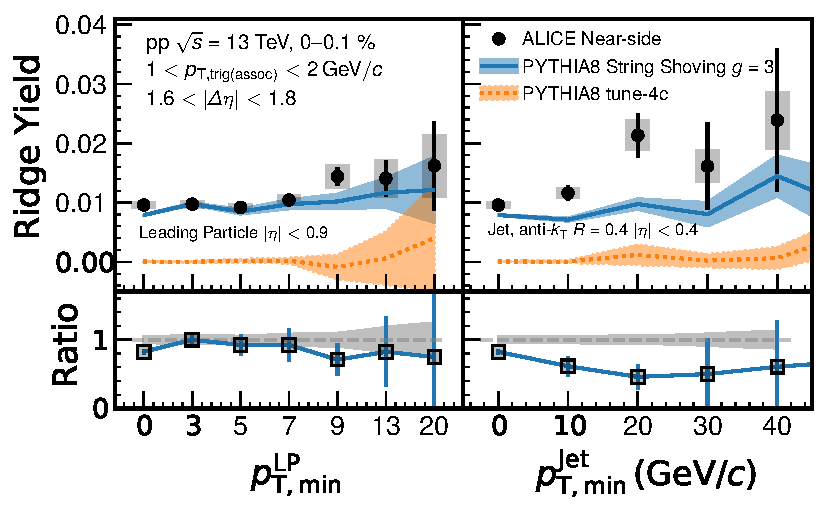
\includegraphics[width=0.99\linewidth]{./figures/Fig6_RidgeYieldESE.pdf}
	\caption{The ridge yield spectra with respect to the leading particle and jet selections. The filled circles show measurement with ALICE. Model predictions are compared with measurement as blue line for $\pythiashoving$ and orange line for $\pythiam$.}
	\label{fig:RidgeYield_ESE}
\end{figure}



